\documentclass{beamer}
\usepackage{ulem}
\usepackage{tikz}
\usepackage{booktabs}
\usepackage{graphicx,threeparttable,caption}
\usetikzlibrary{shapes,snakes}
\usepackage[beamer,customcolors]{hf-tikz}
\usepackage{nicematrix}
\usepackage{xcolor}
\usepackage{makecell}
\usepackage{array}
\usepackage{csquotes}
\usepackage{csquotes}
\usepackage{minted}
\captionsetup{labelformat=empty,labelsep=none}

\graphicspath{ {./png/} }

\usetikzlibrary{
    arrows,
    arrows.meta,
    shapes,
    positioning,
    shadows,
    trees,
    calc
}

\tikzset{%
    >={Latex[width=2mm,length=2mm]},
    % Specifications for style of nodes:
    plain/.style = {},
    base/.style = {
        plain,
        rectangle, rounded corners, draw=black,
        minimum width=1cm, minimum height=1cm,
        text centered, font=\sffamily\tiny\bfseries,
        fill=white, align=center
    },
    app/.style = {base, ellipse},
    data/.style = {base, fill=gray!30},
    action/.style = {base, circle, fill=red!30},
    note/.style = {app, fill=yellow},
    hl/.style={
    set fill color=red!80!black!40,
    set border color=red!80!black
    }
}


\AtBeginSection[]{
  \begin{frame}
  \vfill
  \centering
  \begin{beamercolorbox}[sep=8pt,center,shadow=true,rounded=true]{title}
    \usebeamerfont{title}\insertsectionhead\par%
  \end{beamercolorbox}
  \vfill
  \end{frame}
}
\setbeamercolor{alerted text}{fg=red}
%\usecolortheme[orchid]{structure}
\usetheme[hideothersubsections]{PaloAlto}
\makeatletter
\patchcmd{\csq@bquote@i}{{#6}}{{\emph{#6}}}{}{}
\makeatother
%\usecolortheme{orchid}
%\usefonttheme{professionalfonts}
\newcommand{\soutthick}[1]{%
   \textcolor{red}{
   \renewcommand{\ULthickness}{1pt}%
      \sout{#1}%
   \renewcommand{\ULthickness}{.4pt}% Resetting to ulem default
   }
}
\newcommand{\centered}[1]{\begin{tabular}{l} #1 \end{tabular}}
\setbeamertemplate{section in toc}[square]
\setbeamertemplate{subsection in toc}[square]
\setbeamertemplate{section in sidebar}[shaded]
\setbeamertemplate{items}[square]
\setbeamercovered{transparent} 

\title[]{Introduction to Computational Social Science}
\subtitle{Networks -- how small is the world?}
\author[]{Mikołaj Biesaga\\ \small{\color{blue}{\href{mailto:m.biesaga@uw.edu.pl}{m.biesaga@uw.edu.pl}}}}
\institute{
\includegraphics[width = 4 cm]{uw.png}}
\date{April 8, 2025}
\begin{document}
\begin{frame}
   \titlepage
\end{frame}

\begin{frame}
   \frametitle{Before we start}
   \begin{figure}
      \centering
      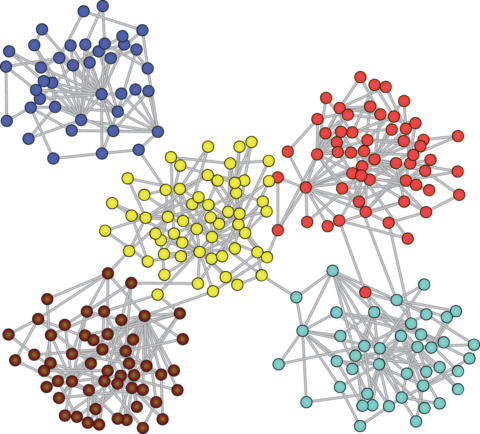
\includegraphics[width = .7\textwidth]{network.png}
      \caption{from \href{https://interactioninstitute.org/network-analysis-for-change-collaborations-clusters-champions-and-coach-weavers/}{\textcolor{blue}{Ogden, 2020}}}
   \end{figure}

\end{frame}

\begin{frame}
   \frametitle{The small world problem}
   \framesubtitle{Milgram, 1967}
   \only<1>{
      \centering{
         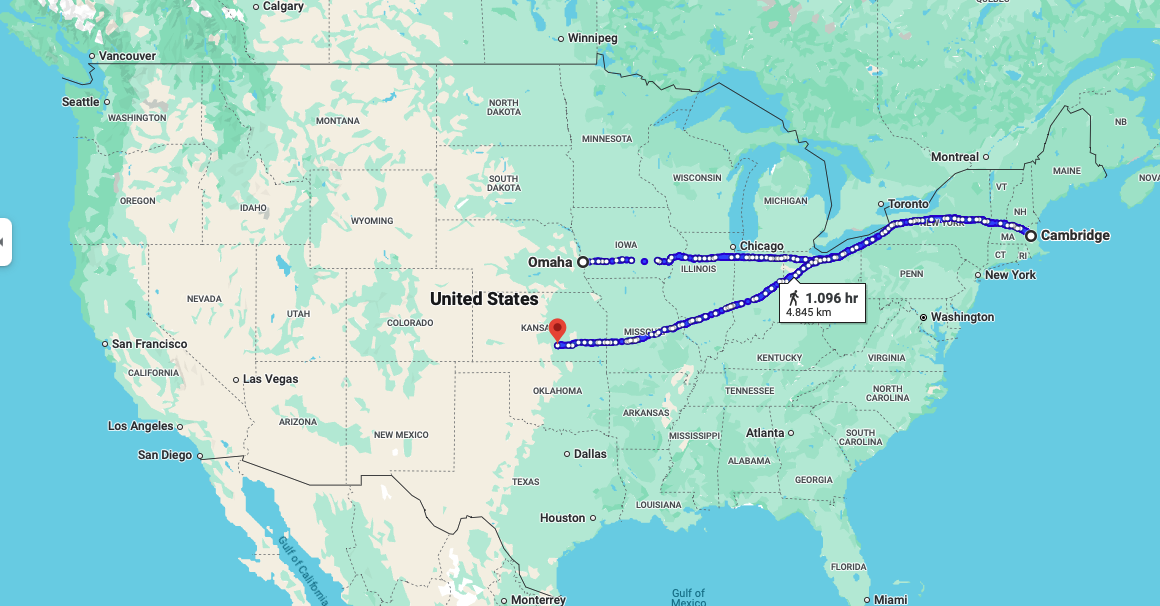
\includegraphics[width = \textwidth]{milgram.png}
      }
   }
   \only<2>{
      \begin{enumerate}
         \item The article was written in 1960s that is why it uses
         \href{https://en.wikipedia.org/wiki/Negro}{\textcolor{blue}{offensive (out-dated) language}}.
         \item What are the two general philosophical views of the small world
         problem?
         \item What are the problems with Milgram's study?
      \end{enumerate}
   }
\end{frame}

\begin{frame}
   \frametitle{How small is the world really?}
   \only<1,2,3>{
      \begin{itemize}
         \item Could it be a big world after all? (Kleinfeld, 2002)
         \only<2>{
            \begin{enumerate}
               \item Only small percentage of packages reached the final destination (Kansas -- 5\%; Nebraska -- 30\%) 
               \item Not a representative sample -- the recruitment process favored 
               sociable people
               \item Social class separation -- low-income senders were only able
               to reach low-income recipients
            \end{enumerate}
         }
         \item How small is the world really? (Dodds, Muhamad, \& Watts, 2003; Goel, Muhamad, \& Watts, 2009)
         \only<3>{
            \begin{enumerate}
               \item Facebook degrees of separation -- 4.57 (Edunov et al., 2016)
               \item Algorithmic vs. topological approach to the small world problem
            \end{enumerate}
         }
      \end{itemize}
   }
   \only<4>{
      \begin{block}{Topological approach}
         The small world problem is a property of the network. The degree of 
         separation refers to the underling structure of the network.
      \end{block}
      \begin{block}{Algorithmic approach}
         The small world problem is a property of the algorithm. The degree of separation refers to the ability (algorithm) to find the shortest path between two nodes.
      \end{block}
   }

\end{frame}

\begin{frame}
   \frametitle{Six degrees of separation}
   \centering
   
\includegraphics[width = .7\textwidth]{png/bacon.png}
\end{frame}

\begin{frame}
   \frametitle{The small world network}
   \only<1>{
      \begin{figure}
         \centering
         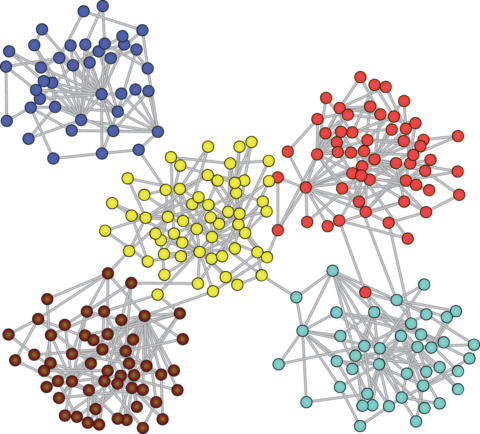
\includegraphics[width = .7\textwidth]{network.png}
         \caption{from \href{https://interactioninstitute.org/network-analysis-for-change-collaborations-clusters-champions-and-coach-weavers/}{\textcolor{blue}{Ogden, 2020}}}
      \end{figure}
   }
   \only<2>{
      \framesubtitle{Homophily}
      \begin{block}{Homophily}
         \underline{Homophily} is a concept in sociology describing the tendency of individuals to associate and bond with similar others, as in the proverb "birds of a feather flock together".
      \end{block}
   }
   \only<3>{
      \framesubtitle{Homophily}
      \begin{figure}
         \centering
         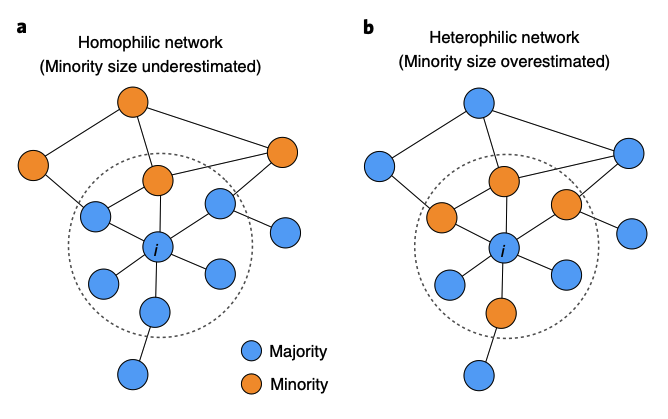
\includegraphics[width = \textwidth]{homophily.png}
         \caption{Lee et al. (2019)}
      \end{figure}
   }
   \only<4>{
      \framesubtitle{Lee et al. (2019)}
      \begin{itemize}
         \item When homophily is \alert{high}, both minority and majority groups
         tend to \alert{overestimate} their own size, whereas when homophily is
         \alert{low}, both groups tend to \alert{underestimate} their own size.
         \item The \alert{smaller the size of the minority group}, the more
         its size is \alert{overestimated} by both minority and majority groups.
      \end{itemize}
   }
\end{frame}

\begin{frame}
   \frametitle{The power of weak ties}

\end{frame}

\begin{frame}
    \frametitle{For the class in two weeks}
    \begin{itemize}
        \item Nowak, A., Rychwalska, A., \& Borkowski, W. (2013). Why Simulate?
        To Develop a Mental Model. Journal of Artificial Societies and Social
        Simulation, 16(3), 12.
        \href{https://doi.org/10.18564/jasss.2235}{\textcolor{blue}{https://doi.org/10.18564/jasss.2235}}.
    \end{itemize}
\end{frame}

\end{document}